\documentclass[12pt]{article}
\usepackage{graphicx}
\usepackage{subcaption}
\usepackage{mwe}
\usepackage[]{mcode}
%\usepackage{lingmacros}
%\usepackage{tree-dvips}
%\usepackage{blindtext}
%\usepackage[utf8]{inputenc}

\begin{document}

\title{CMSC 426 - HW1}
\author{Gudjon Einar Magnusson}

\maketitle

\section{Blobs}

\subsection{My Region Props}

\subsubsection{Area}
\begin{minipage}{\linewidth}
\begin{lstlisting}
    %% Count number of pixesl in blob
    stats(count).Area = sum(sum(CurrBlob));
\end{lstlisting}
\end{minipage}

\subsubsection{Centroid}
\begin{minipage}{\linewidth}
\begin{lstlisting}
    %% Find index of non-zero elements
    [r, c] = find(CurrBlob);
    n = size(r, 1);
    %% Compute avarege of all non-zero pixel coordinates
    stats(count).Centroid = [sum(c)/n, sum(r)/n];
\end{lstlisting}
\end{minipage}

\subsubsection{Bounding Box}
\begin{minipage}{\linewidth}
\begin{lstlisting}
    %% Find index of non-zero elements
    [r, c] = find(CurrBlob);
    %% Find bounds and add padding
    maxCol = max(c) + 0.5;
    minCol = min(c) - 0.5;
    maxRow = max(r) + 0.5;
    minRow = min(r) - 0.5;
    stats(count).BoundingBox = [minCol, minRow, maxCol-minCol, maxRow-minRow];
\end{lstlisting}
\end{minipage}


\subsection{Fill Holes}


\section{Gabor Filters}

\section{}

\section{}

\section{}

\section{Seam Carving}

For the seam carving algorithm I use an energy function that is simply the gradient of each pixel. The gradient is calculated by applying the \textit{imgradient} function on a grayscale version of the image.

Unfortunately my seam carving implementation is not very optimized, so to save some time reduced the size of the sample image by 50\%.
In figure \ref{fig_carve} you can see the result of carving 50 horizontal and 100 vertical seams from the sample image. Overall the results are descent but unfortunately the person in the picture is cut in half, this is the most notable flaw. 


\begin{figure}
    \begin{subfigure}[t]{.49\textwidth}
        \centering
        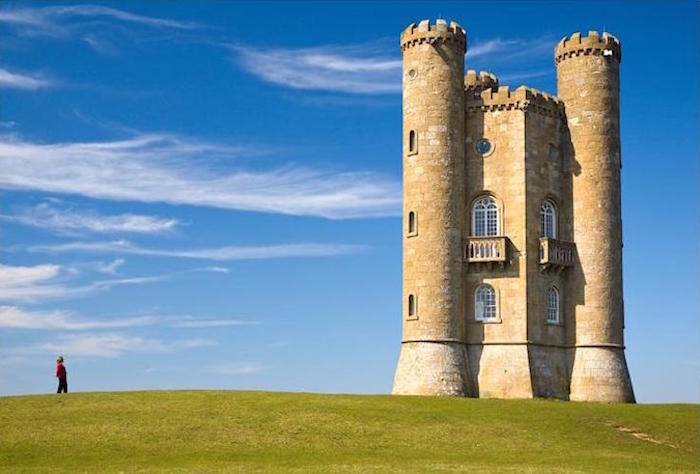
\includegraphics[width=\linewidth]{carving_original}
    \end{subfigure}\hfill
    \begin{subfigure}[t]{.47\textwidth}
        \centering
        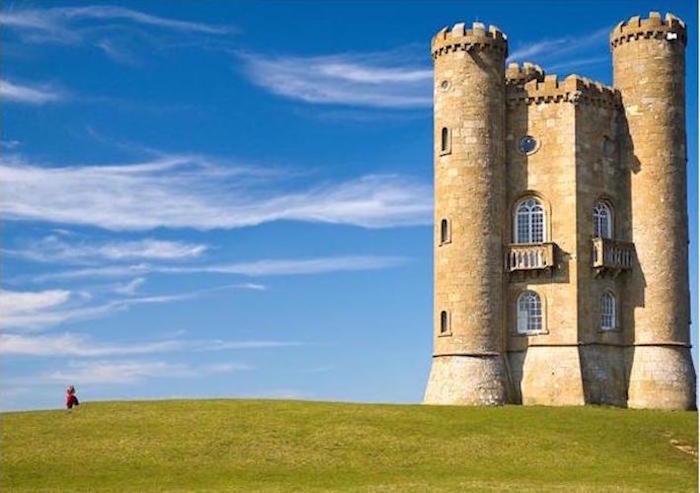
\includegraphics[width=\linewidth]{carving_50_100}
    \end{subfigure}
    \caption{Before and after seam carving}
    \label{fig_carve}
\end{figure}

\end{document}